\documentclass{article}
\usepackage{amsmath}
\usepackage{graphicx}

\title{Proyecto Laboratorio Redes}
\author{Roberto Andrés Alvarado Moreira}

\begin{document}
\maketitle
\section{Resultados}%

Para el subnetting de esta red se utilizó el metodo VLSM,
donde cada subnet esta definida por la cantidad de
dispostivos que necesita, solo se hará primeramente para
Gaias y los demás siguen el mismo proceso, 
entonces vamos  tener como refencia la tabla de subnetting  

\begin{figure}[h]
\begin{center}
  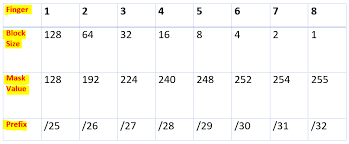
\includegraphics[scale=0.8]{image1.png}
\end{center}
\end{figure}
En este caso necesitamos 900 direcciones entonces, tomamos 
$$2^{10} = 1024 \geq 900 $$
Como tenemos la dirección 172.21.0.0/16 que es Clase B, entonces vamos a tomar
de los 16 bits disponibles 10, por lo que se tiene que son 6 bits que se van a
seleccionar, entonces el prefijo que se va a utilizar es /22. Asi con los otros
en la tabla se ven los resultados para todos los demás


\newpage
\begin{table}[h]
  \caption{Table de Resultados de direcciones}
  \label{tab:}
  \begin{center}
    \begin{tabular}[c]{l|l}
      \hline
      \multicolumn{1}{c|}{\textbf{}} & 
      \multicolumn{1}{c}{\textbf{}} \\
      \hline
       Gaias   & 172.21.0.0/22 \\
       GYE     & 172.21.4.0/24 \\
       HDLV    & 172.21.5.0/25 \\
       Gaias-U & 172.21.5.128/30 \\
       GYE-U   & 172.21.5.132/30 \\
       HDLV-U  & 172.21.5.136/30 \\
      \hline
    \end{tabular}
  \end{center}
\end{table}
 
\begin{table}[h]
  \caption{Table de Resultados de submascaras}
  \label{tab:}
  \begin{center}
    \begin{tabular}[c]{l|l}
      \hline
      \multicolumn{1}{c|}{\textbf{}} & 
      \multicolumn{1}{c}{\textbf{}} \\
      \hline
       Gaias   & 255.255.252.0 \\
       GYE     & 255.255.255.0 \\
       HDLV    & 255.255.255.128 \\
       Gaias-U & 255.255.255.252 \\
       GYE-U   & 255.255.255.252 \\
       HDLV-U  & 255.255.255.252 \\
      \hline
    \end{tabular}
  \end{center}
\end{table}
\end{document}
